\begin{pastexam}[label={px:ntut-113-ee-ds-06}]{北科大電機所（戊組）113 學年度 第 II.2 題}
（簡答；4 分）

Given a binary search tree in Fig. 1, insert 27, 15, 63, 99, 70, and 85 (in this order) into the
binary search tree. What is the post-order traversal? (4\%)

\begin{center}
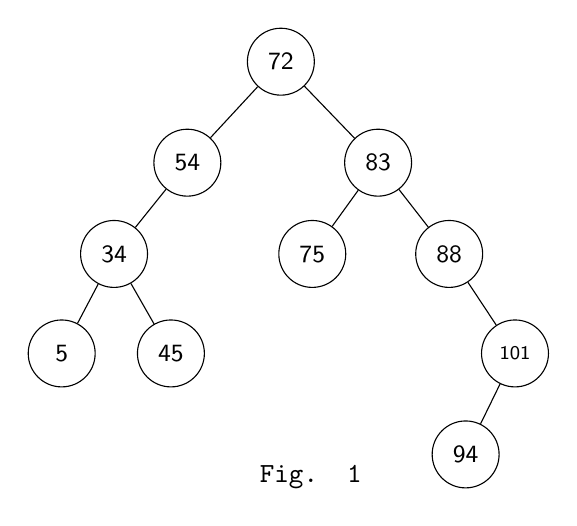
\begin{tikzpicture}[x=0.95cm,y=-0.95cm,
  v/.style={circle,draw,inner sep=0pt,minimum size=8.5mm,font=\sffamily\small}]
\node[v] (n72) at (3.80,0.80) {72};
\node[v] (n54) at (2.55,2.15) {54};
\node[v] (n83) at (5.10,2.15) {83};
\node[v] (n34) at (1.57,3.37) {34};
\node[v] (n75) at (4.22,3.37) {75};
\node[v] (n88) at (6.05,3.37) {88};
\node[v] (n5) at (0.87,4.70) {5};
\node[v] (n45) at (2.33,4.70) {45};
\node[v] (n101) at (6.93,4.70) {\scriptsize 101};
\node[v] (n94) at (6.27,6.05) {94};
\draw (n72) -- (n54) (n72) -- (n83) (n54) -- (n34) (n34) -- (n5) (n34) -- (n45)
      (n83) -- (n75) (n83) -- (n88) (n88) -- (n101) (n101) -- (n94);
\node[font=\ttfamily\bfseries] at (4.2,6.35) {Fig. 1};
\end{tikzpicture}
\end{center}
\end{pastexam}

\begin{pastsoln}
答案：15, 27, 5, 45, 34, 70, 63, 54, 75, 85, 99, 94, 101, 88, 83, 72。

\textbf{插入}（資結書第~9.2~節）。 每個鍵從根往下比：小於節點往左、大於往右，走到空的位置就
放下。
\begin{itemize}
\item $27$：$27 < 72$ 左，$< 54$ 左，$< 34$ 左，$> 5$ 右；$5$ 的右邊是空的，放在 $5$ 的右子節點。
\item $15$：$72$ 左、$54$ 左、$34$ 左、$5$ 右，到 $27$；$15 < 27$ 左，放在 $27$ 的左子節點。
\item $63$：$63 < 72$ 左，$63 > 54$ 右；$54$ 的右邊是空的，放在 $54$ 的右子節點。
\item $99$：$> 72$ 右，$> 83$ 右，$> 88$ 右，$< 101$ 左，到 $94$；$99 > 94$，放在 $94$ 的右子節點。
\item $70$：$72$ 左，$54$ 右，到 $63$；$70 > 63$，放在 $63$ 的右子節點。
\item $85$：$72$ 右，$83$ 右，到 $88$；$85 < 88$，放在 $88$ 的左子節點。
\end{itemize}
插入後的樹如下（灰底是新插入的節點）：
\begin{center}
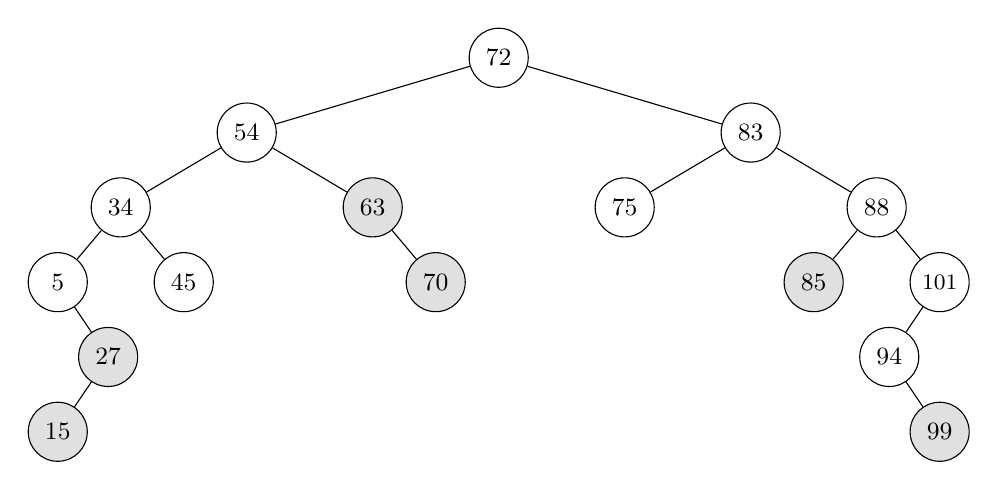
\begin{tikzpicture}[x=0.8cm, y=-0.95cm,
  v/.style={circle,draw,inner sep=0pt,minimum size=7.5mm,font=\small},
  nw/.style={v, fill=black!12}]
\node[v] (72) at (8,0) {72};
\node[v] (54) at (4,1) {54};
\node[v] (83) at (12,1) {83};
\node[v] (34) at (2,2) {34};
\node[nw] (63) at (6,2) {63};
\node[v] (75) at (10,2) {75};
\node[v] (88) at (14,2) {88};
\node[v] (5) at (1,3) {5};
\node[v] (45) at (3,3) {45};
\node[nw] (70) at (7,3) {70};
\node[nw] (85) at (13,3) {85};
\node[v] (101) at (15,3) {\footnotesize 101};
\node[nw] (27) at (1.8,4) {27};
\node[v] (94) at (14.2,4) {94};
\node[nw] (15) at (1.0,5) {15};
\node[nw] (99) at (15,5) {99};
\draw (72)--(54) (72)--(83) (54)--(34) (54)--(63) (83)--(75) (83)--(88)
      (34)--(5) (34)--(45) (63)--(70) (88)--(85) (88)--(101)
      (5)--(27) (27)--(15) (101)--(94) (94)--(99);
\end{tikzpicture}
\end{center}

\textbf{後序走訪}（左子樹、右子樹、根；資結書第~7.3~節）。 分段寫：
\begin{itemize}
\item 以 $5$ 為根的子樹：$5$ 沒有左子樹，右子樹是 $27$（左邊接 $15$），得 $15, 27, 5$。
\item 以 $34$ 為根：$15, 27, 5$，再 $45$，再 $34$。
\item 以 $63$ 為根：$70, 63$。
\item 以 $54$ 為根：$15, 27, 5, 45, 34,\ 70, 63,\ 54$。
\item 以 $101$ 為根：左子樹 $94$（右邊接 $99$）得 $99, 94$，再 $101$。
\item 以 $88$ 為根：$85,\ 99, 94, 101,\ 88$。
\item 以 $83$ 為根：$75,\ 85, 99, 94, 101, 88,\ 83$。
\item 整棵：左子樹、右子樹，最後是根 $72$。
\end{itemize}
合起來就是開頭的答案。 檢查：一共 $10 + 6 = 16$ 個鍵，最後一個是根 $72$。
\end{pastsoln}
